\documentclass[conference]{IEEEtran}
\IEEEoverridecommandlockouts

\usepackage{cite}
\usepackage{amsmath,amssymb,amsfonts}
\usepackage{algorithmic}
\usepackage{graphicx}
\usepackage{textcomp}
\usepackage{xcolor}

\def\BibTeX{{\rm B\kern-.05em{\sc i\kern-.025em b}\kern-.08em
    T\kern-.1667em\lower.7ex\hbox{E}\kern-.125emX}}

\begin{document}

\title{Paper Title}

\author{
\IEEEauthorblockN{Naruki Shirahama}
\IEEEauthorblockA{\textit{Shimonoseki City University} \\
Shimonoseki, Yamaguchi, Japan \\
nshirahama@ieee.org}
\and
\IEEEauthorblockN{Yuma Yoshimoto}
\IEEEauthorblockA{\textit{NIT (KOSEN), Kitakyushu College} \\
Kitakyushu, Fukuoka, Japan \\
yoshimoto@kct.ac.jp}
\and
\IEEEauthorblockN{Naofumi Nakaya}
\IEEEauthorblockA{\textit{Juntendo University} \\
Urayasu, Chiba, Japan \\
n.nakaya.ac@juntendo.ac.jp}
\and
\IEEEauthorblockN{Junji Nishino}
\IEEEauthorblockA{\textit{Tamagawa University} \\
Machida, Tokyo, Japan \\
nishinojunji@eng.tamagawa.ac.jp}
\and
\IEEEauthorblockN{Satoshi Watanabe}
\IEEEauthorblockA{\textit{Shizuoka Institute of Science and Technology} \\
Fukuroi, Shizuoka, Japan \\
satoshi\_watanabe@ieee.org}
}

\maketitle

\begin{abstract}
Write the abstract here.
\end{abstract}

\begin{IEEEkeywords}
keyword1, keyword2, keyword3
\end{IEEEkeywords}

\section{Introduction}

\section{Related Work}

\section{Method}
\begin{figure}[t]
\centering
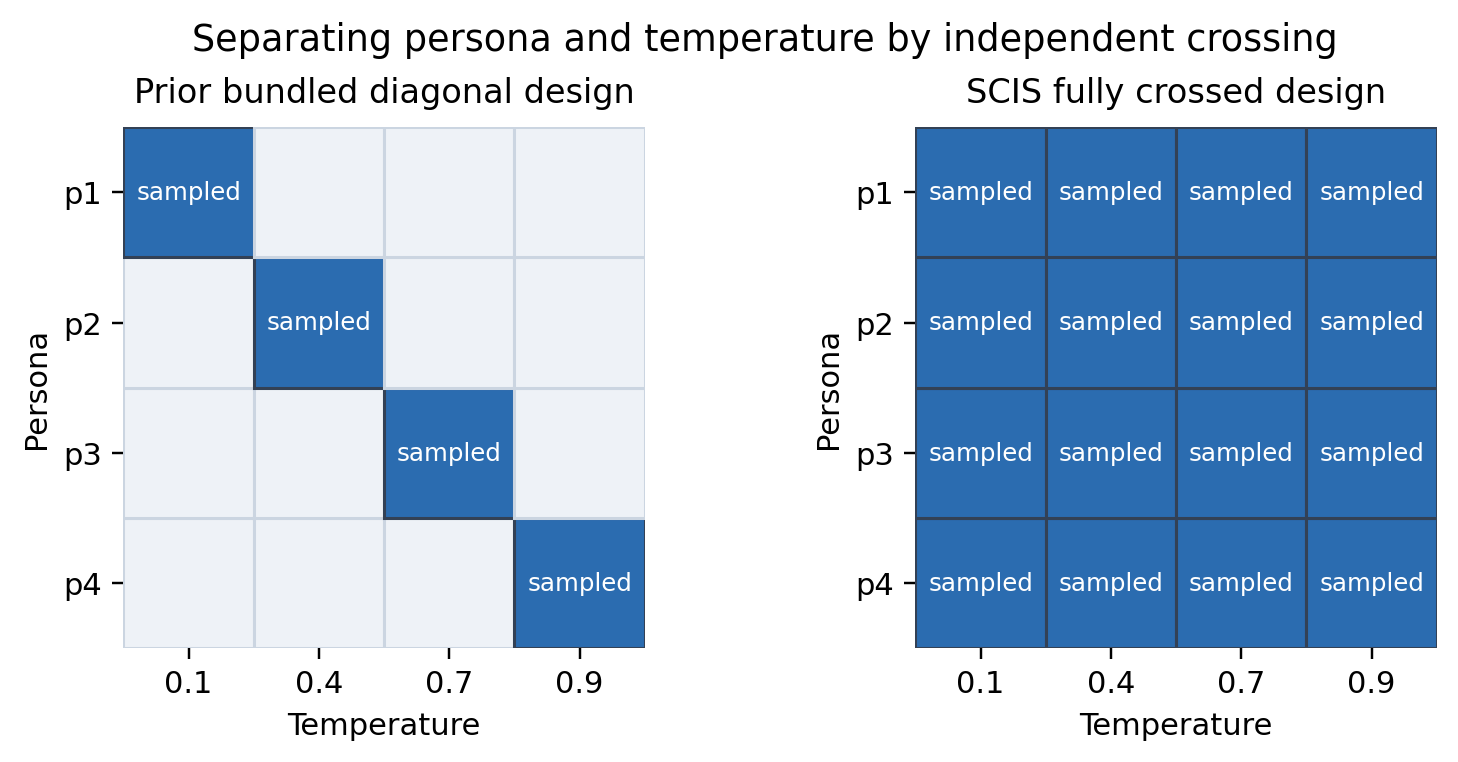
\includegraphics[width=\linewidth]{../../artifacts/scis2026/main_figures_v1/figure1_design_comparison.png}
\caption{Prior diagonal persona-temperature bundles are contrasted with the SCIS fully crossed persona x temperature design.}
\label{fig:scis-design}
\end{figure}


\section{Experiments}
\begin{table}[t]
\centering
\caption{SCIS main-run validity and completeness.}
\label{tab:scis-validity}
\begin{tabular}{rrrrrr}
\hline
Resp. & Valid & Rate & Emo. rows & Miss. scores & Miss. cells \\
\hline
1440 & 1440 & 100.0\% & 5760 & 0 & 0 \\
\hline
\end{tabular}
\end{table}


\section{Results and Discussion}
\begin{table*}[t]
\centering
\caption{Balanced persona-temperature effect decomposition by metric and emotion. Entropy rows use the primary sigmoid-S membership family.}
\label{tab:scis-effect-summary}
\begin{tabular}{llrrrrr}
\hline
Metric & Emotion & $n$ & Persona & Temp. & Interaction & Separability \\
\hline
Entropy $H^*$ & Anger & 18 & 61.0\% & 10.7\% & 28.3\% & 71.7\% \\
Entropy $H^*$ & Interest & 18 & 81.7\% & 4.8\% & 13.5\% & 86.5\% \\
Entropy $H^*$ & Sadness & 18 & 87.1\% & 3.4\% & 9.6\% & 90.4\% \\
Entropy $H^*$ & Surprise & 18 & 73.3\% & 6.9\% & 19.8\% & 80.2\% \\
Score & Anger & 18 & 80.8\% & 6.0\% & 13.2\% & 86.8\% \\
Score & Interest & 18 & 93.7\% & 1.8\% & 4.6\% & 95.4\% \\
Score & Sadness & 18 & 95.3\% & 1.3\% & 3.4\% & 96.6\% \\
Score & Surprise & 18 & 90.0\% & 3.0\% & 7.0\% & 93.0\% \\
\hline
\end{tabular}
\end{table*}

\begin{figure}[t]
\centering
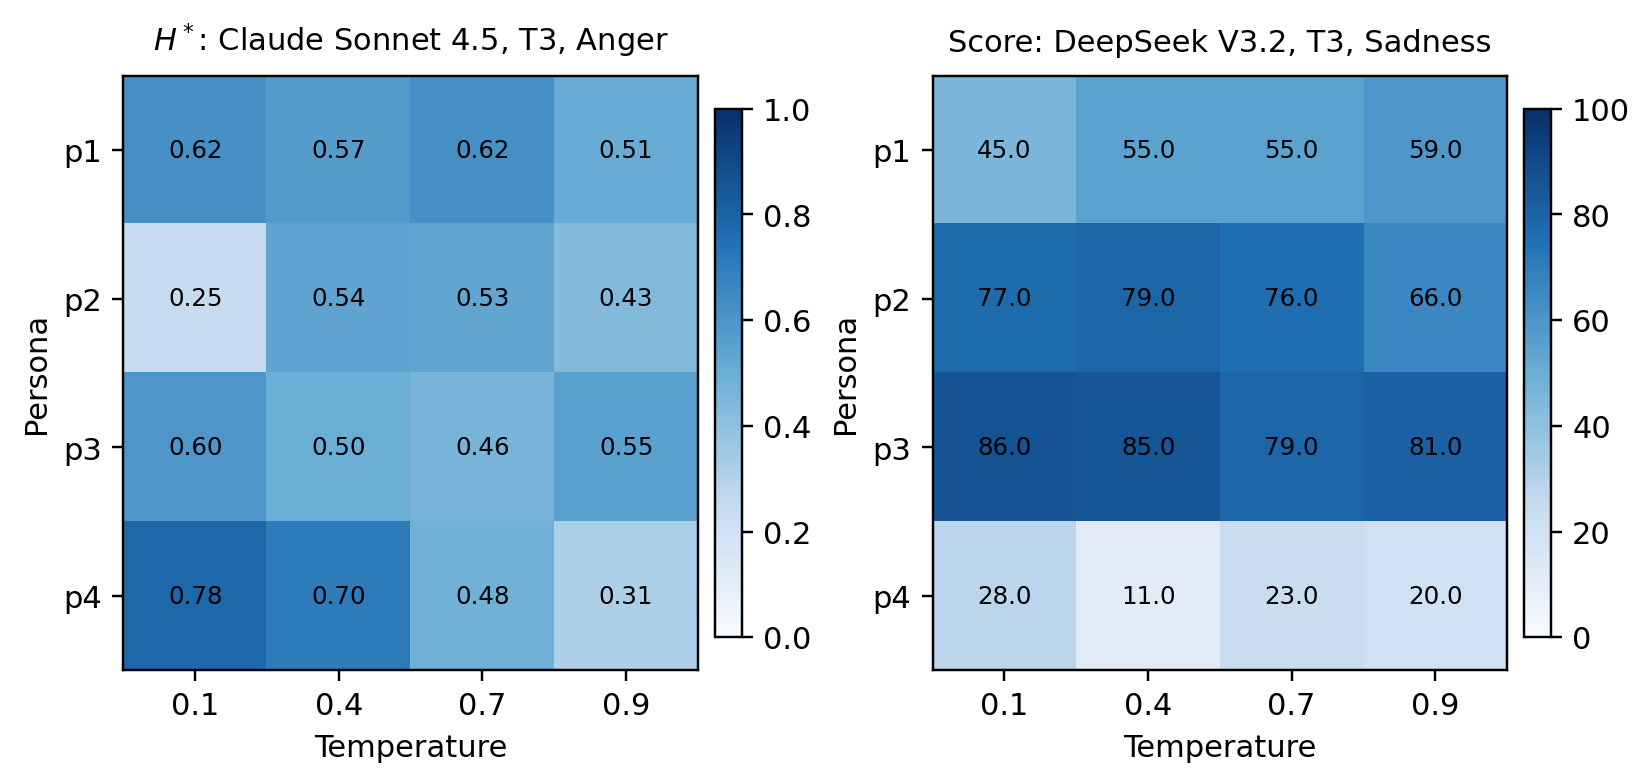
\includegraphics[width=\linewidth]{../../artifacts/scis2026/main_figures_v1/figure2_representative_heatmaps.png}
\caption{H\_norm\_sigmoid\_s\_v1 anthropic/claude-sonnet-4.5 T3 anger burden=0.654771; score deepseek/deepseek-v3.2 T3 sadness burden=0.039432}
\label{fig:scis-representative-heatmaps}
\end{figure}

\begin{table*}[t]
\centering
\caption{Model-level mean decomposition shares by metric.}
\label{tab:scis-model-summary}
\begin{tabular}{llrrrrr}
\hline
Model & Metric & $n$ & Persona & Temp. & Mean int. & Max int. \\
\hline
Claude Sonnet 4.5 & Entropy $H^*$ & 12 & 87.1\% & 2.8\% & 10.1\% & 65.5\% \\
Claude Sonnet 4.5 & Score & 12 & 98.2\% & 0.5\% & 1.3\% & 2.8\% \\
DeepSeek V3.2 & Entropy $H^*$ & 12 & 64.7\% & 9.4\% & 25.9\% & 64.8\% \\
DeepSeek V3.2 & Score & 12 & 88.7\% & 4.0\% & 7.4\% & 15.9\% \\
Gemini 2.5 Pro & Entropy $H^*$ & 12 & 65.4\% & 8.6\% & 26.0\% & 60.0\% \\
Gemini 2.5 Pro & Score & 12 & 85.3\% & 4.0\% & 10.7\% & 60.0\% \\
Llama 4 Maverick & Entropy $H^*$ & 12 & 73.5\% & 8.8\% & 17.7\% & 42.5\% \\
Llama 4 Maverick & Score & 12 & 78.3\% & 6.5\% & 15.2\% & 47.4\% \\
GPT-5.4 & Entropy $H^*$ & 12 & 85.6\% & 5.6\% & 8.9\% & 35.4\% \\
GPT-5.4 & Score & 12 & 91.4\% & 2.5\% & 6.0\% & 21.7\% \\
Grok 4.20 & Entropy $H^*$ & 12 & 78.3\% & 3.6\% & 18.2\% & 58.3\% \\
Grok 4.20 & Score & 12 & 97.9\% & 0.6\% & 1.6\% & 4.9\% \\
\hline
\end{tabular}
\end{table*}

\begin{figure}[t]
\centering
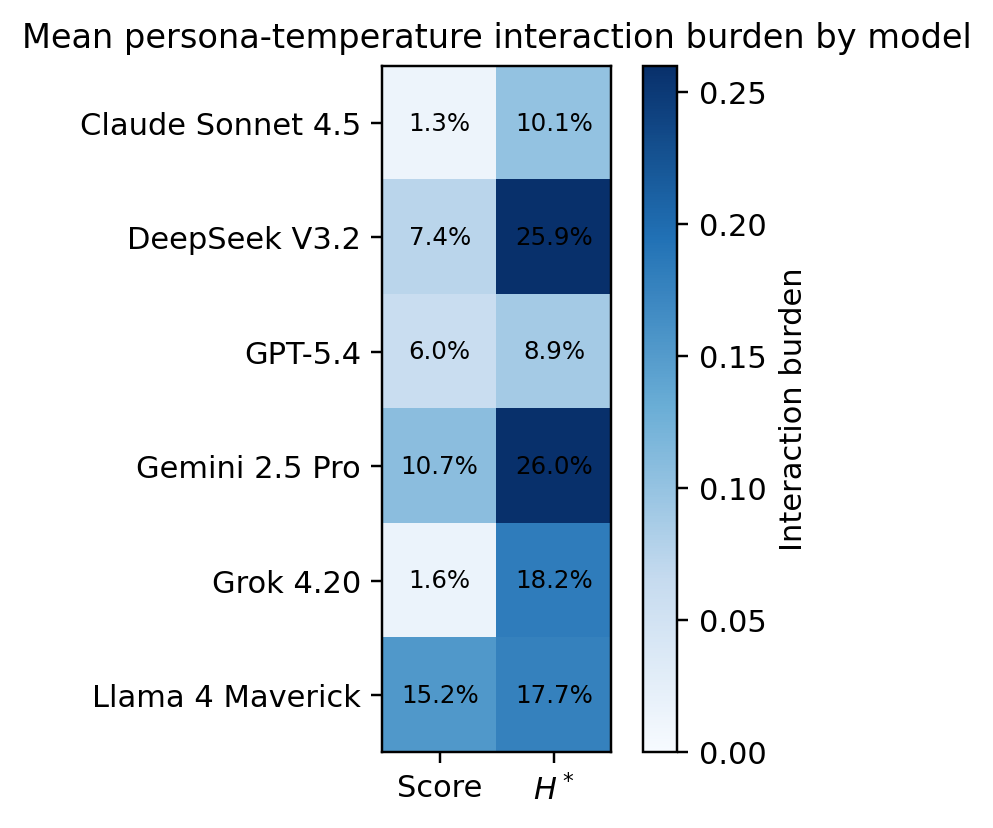
\includegraphics[width=\linewidth]{../../artifacts/scis2026/main_figures_v1/figure3_model_metric_interaction_heatmap.png}
\caption{Mean interaction burden is summarized for score and normalized fuzzy entropy by model.}
\label{fig:scis-model-metric-heatmap}
\end{figure}

\begin{table*}[t]
\centering
\caption{Normalized fuzzy entropy sensitivity to membership-family choice.}
\label{tab:scis-entropy-sensitivity}
\begin{tabular}{llrrrrrr}
\hline
Primary & Baseline & $n$ & $H_{\max}$ P & $H_{\max}$ B & $r$ & Mean $|\Delta|$ & Max $|\Delta|$ \\
\hline
sigmoid\_s\_v1 & legacy\_linear\_v1 & 1152 & 1.019 & 1.058 & 0.933 & 0.130 & 0.479 \\
\hline
\end{tabular}
\end{table*}

\begin{table*}[t]
\centering
\caption{Largest relative and absolute persona-temperature interaction cases.}
\label{tab:scis-top-interactions}
\begin{tabular}{rrlllrrr}
\hline
Type & Rank & Metric & Model & Text & Emotion & SS int. & Burden \\
\hline
relative & 1 & $H^*$ (sigmoid\_s\_v1) & Claude Sonnet 4.5 & T3 & Anger & 0.171 & 65.5\% \\
relative & 2 & $H^*$ (sigmoid\_s\_v1) & DeepSeek V3.2 & T3 & Anger & 0.218 & 64.8\% \\
relative & 3 & Score & Gemini 2.5 Pro & T1 & Anger & 2.250 & 60.0\% \\
relative & 4 & $H^*$ (sigmoid\_s\_v1) & Gemini 2.5 Pro & T1 & Anger & 0.001 & 60.0\% \\
relative & 5 & $H^*$ (sigmoid\_s\_v1) & Grok 4.20 & T3 & Interest & 0.143 & 58.3\% \\
relative & 6 & $H^*$ (sigmoid\_s\_v1) & Gemini 2.5 Pro & T3 & Surprise & 0.225 & 47.4\% \\
relative & 7 & Score & Llama 4 Maverick & T2 & Surprise & 45.000 & 47.4\% \\
relative & 8 & $H^*$ (sigmoid\_s\_v1) & DeepSeek V3.2 & T3 & Surprise & 0.155 & 45.1\% \\
absolute & 1 & Score & DeepSeek V3.2 & T3 & Sadness & 380.062 & 3.9\% \\
absolute & 2 & Score & DeepSeek V3.2 & T3 & Anger & 362.750 & 15.9\% \\
absolute & 3 & Score & Gemini 2.5 Pro & T3 & Surprise & 292.500 & 4.9\% \\
absolute & 4 & Score & Gemini 2.5 Pro & T1 & Interest & 282.562 & 8.4\% \\
\hline
\end{tabular}
\end{table*}


\section{Conclusion}

\section*{Acknowledgment}

% Add references when needed, for example:
% \begin{thebibliography}{00}
% \bibitem{ref1} Author, ``Title,'' Journal or Conference, year.
% \end{thebibliography}

\end{document}
